\section{Lattice and optics interaction}
\label{sec:optics}

The lattice helper parses PTC flat-file fibre blocks and exposes one-based fibre indices, element names, lengths, and source line spans. Name resolution first looks for an exact element-name match, then supports a parent dipole name expanding to numbered sliced dipole records. This is a parser contract for the flat-file form, not a general MAD-X sequence parser. [claim:LATTICE-02]

After lattice initialization and Twiss update, users can query tunes, chromaticities, phase advances, and per-node Twiss/orbit data through \texttt{PTC}. The code returns values and field names; physical coordinate meaning, unit conventions, and validity ranges are separate review questions. Do not infer them from names alone. [claim:API-04]

\begin{figure}[ht]
  \centering
  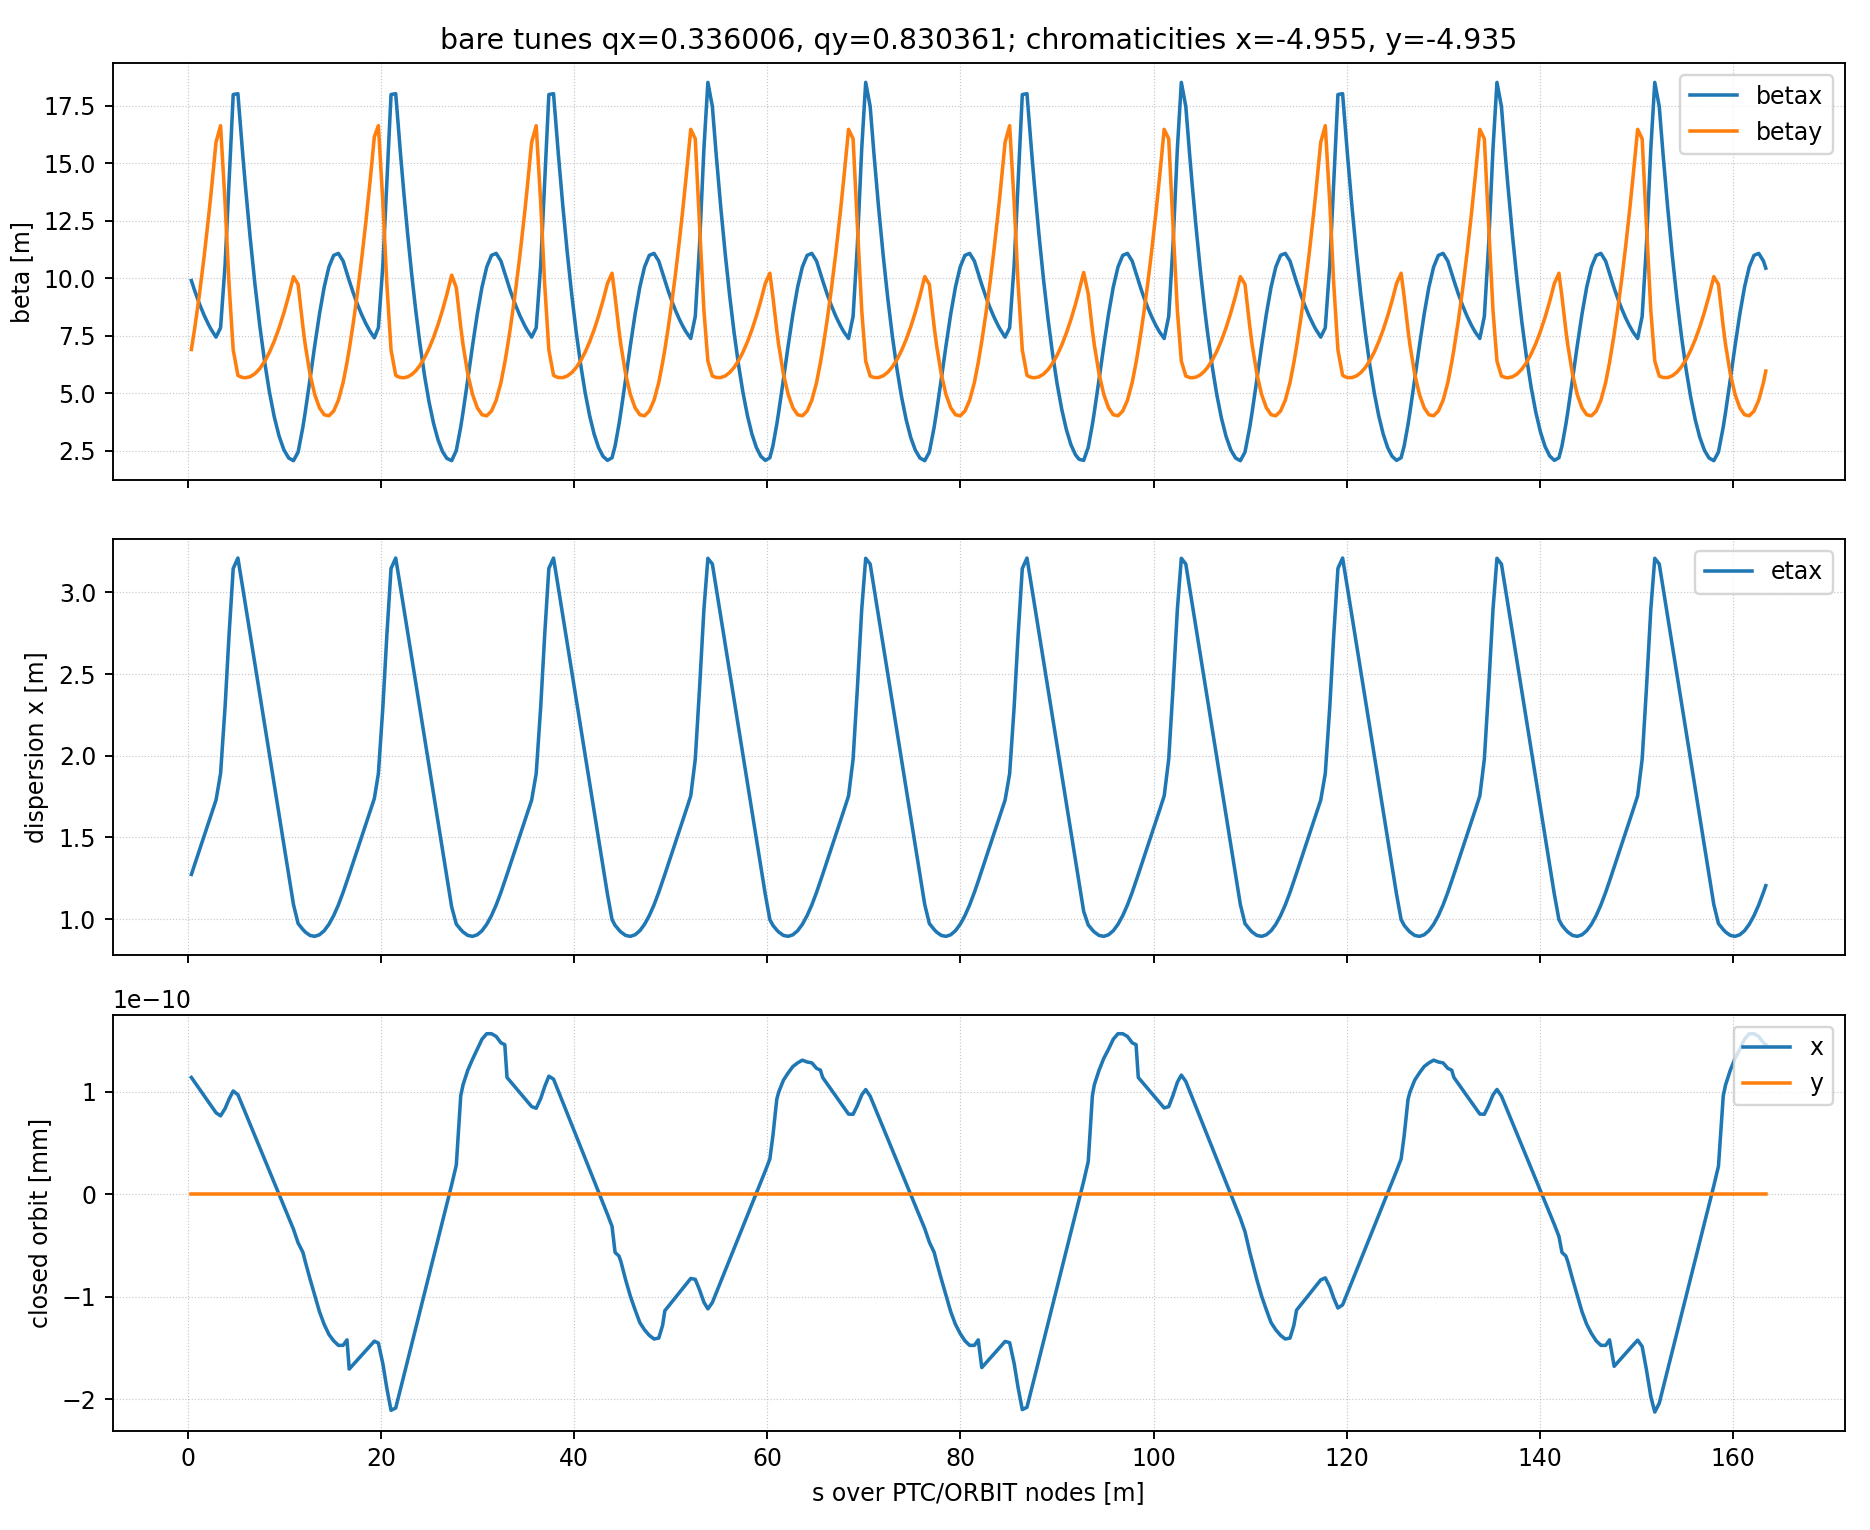
\includegraphics[width=0.96\textwidth]{figures/bare_twiss_closed_orbit.png}
  \caption{Repository optics diagnostic generated by the bare optics example. The copied pixels are unchanged. It illustrates the plotted fields available from this example; it is not a comparison to a reference model or physics acceptance. [claim:PROV-03]}
\end{figure}

\subsection{One-turn maps and normal forms}

\texttt{one\_turn\_map()} and \texttt{normal\_form()} both raise the not-exposed exception. [claim:LIMIT-01]
